% !TEX root = MATLAB_Introduction_Blair.tex
\section{Using MATLAB}

In this section, we describe how to begin using MATLAB.

% ============================================
% ============================================
\subsection{The MATLAB User Interface}

% vvv------------------------------------------------------------vvv
\begin{figure}[htbp] %  figure placement: here, top, bottom, or page
   \centering
   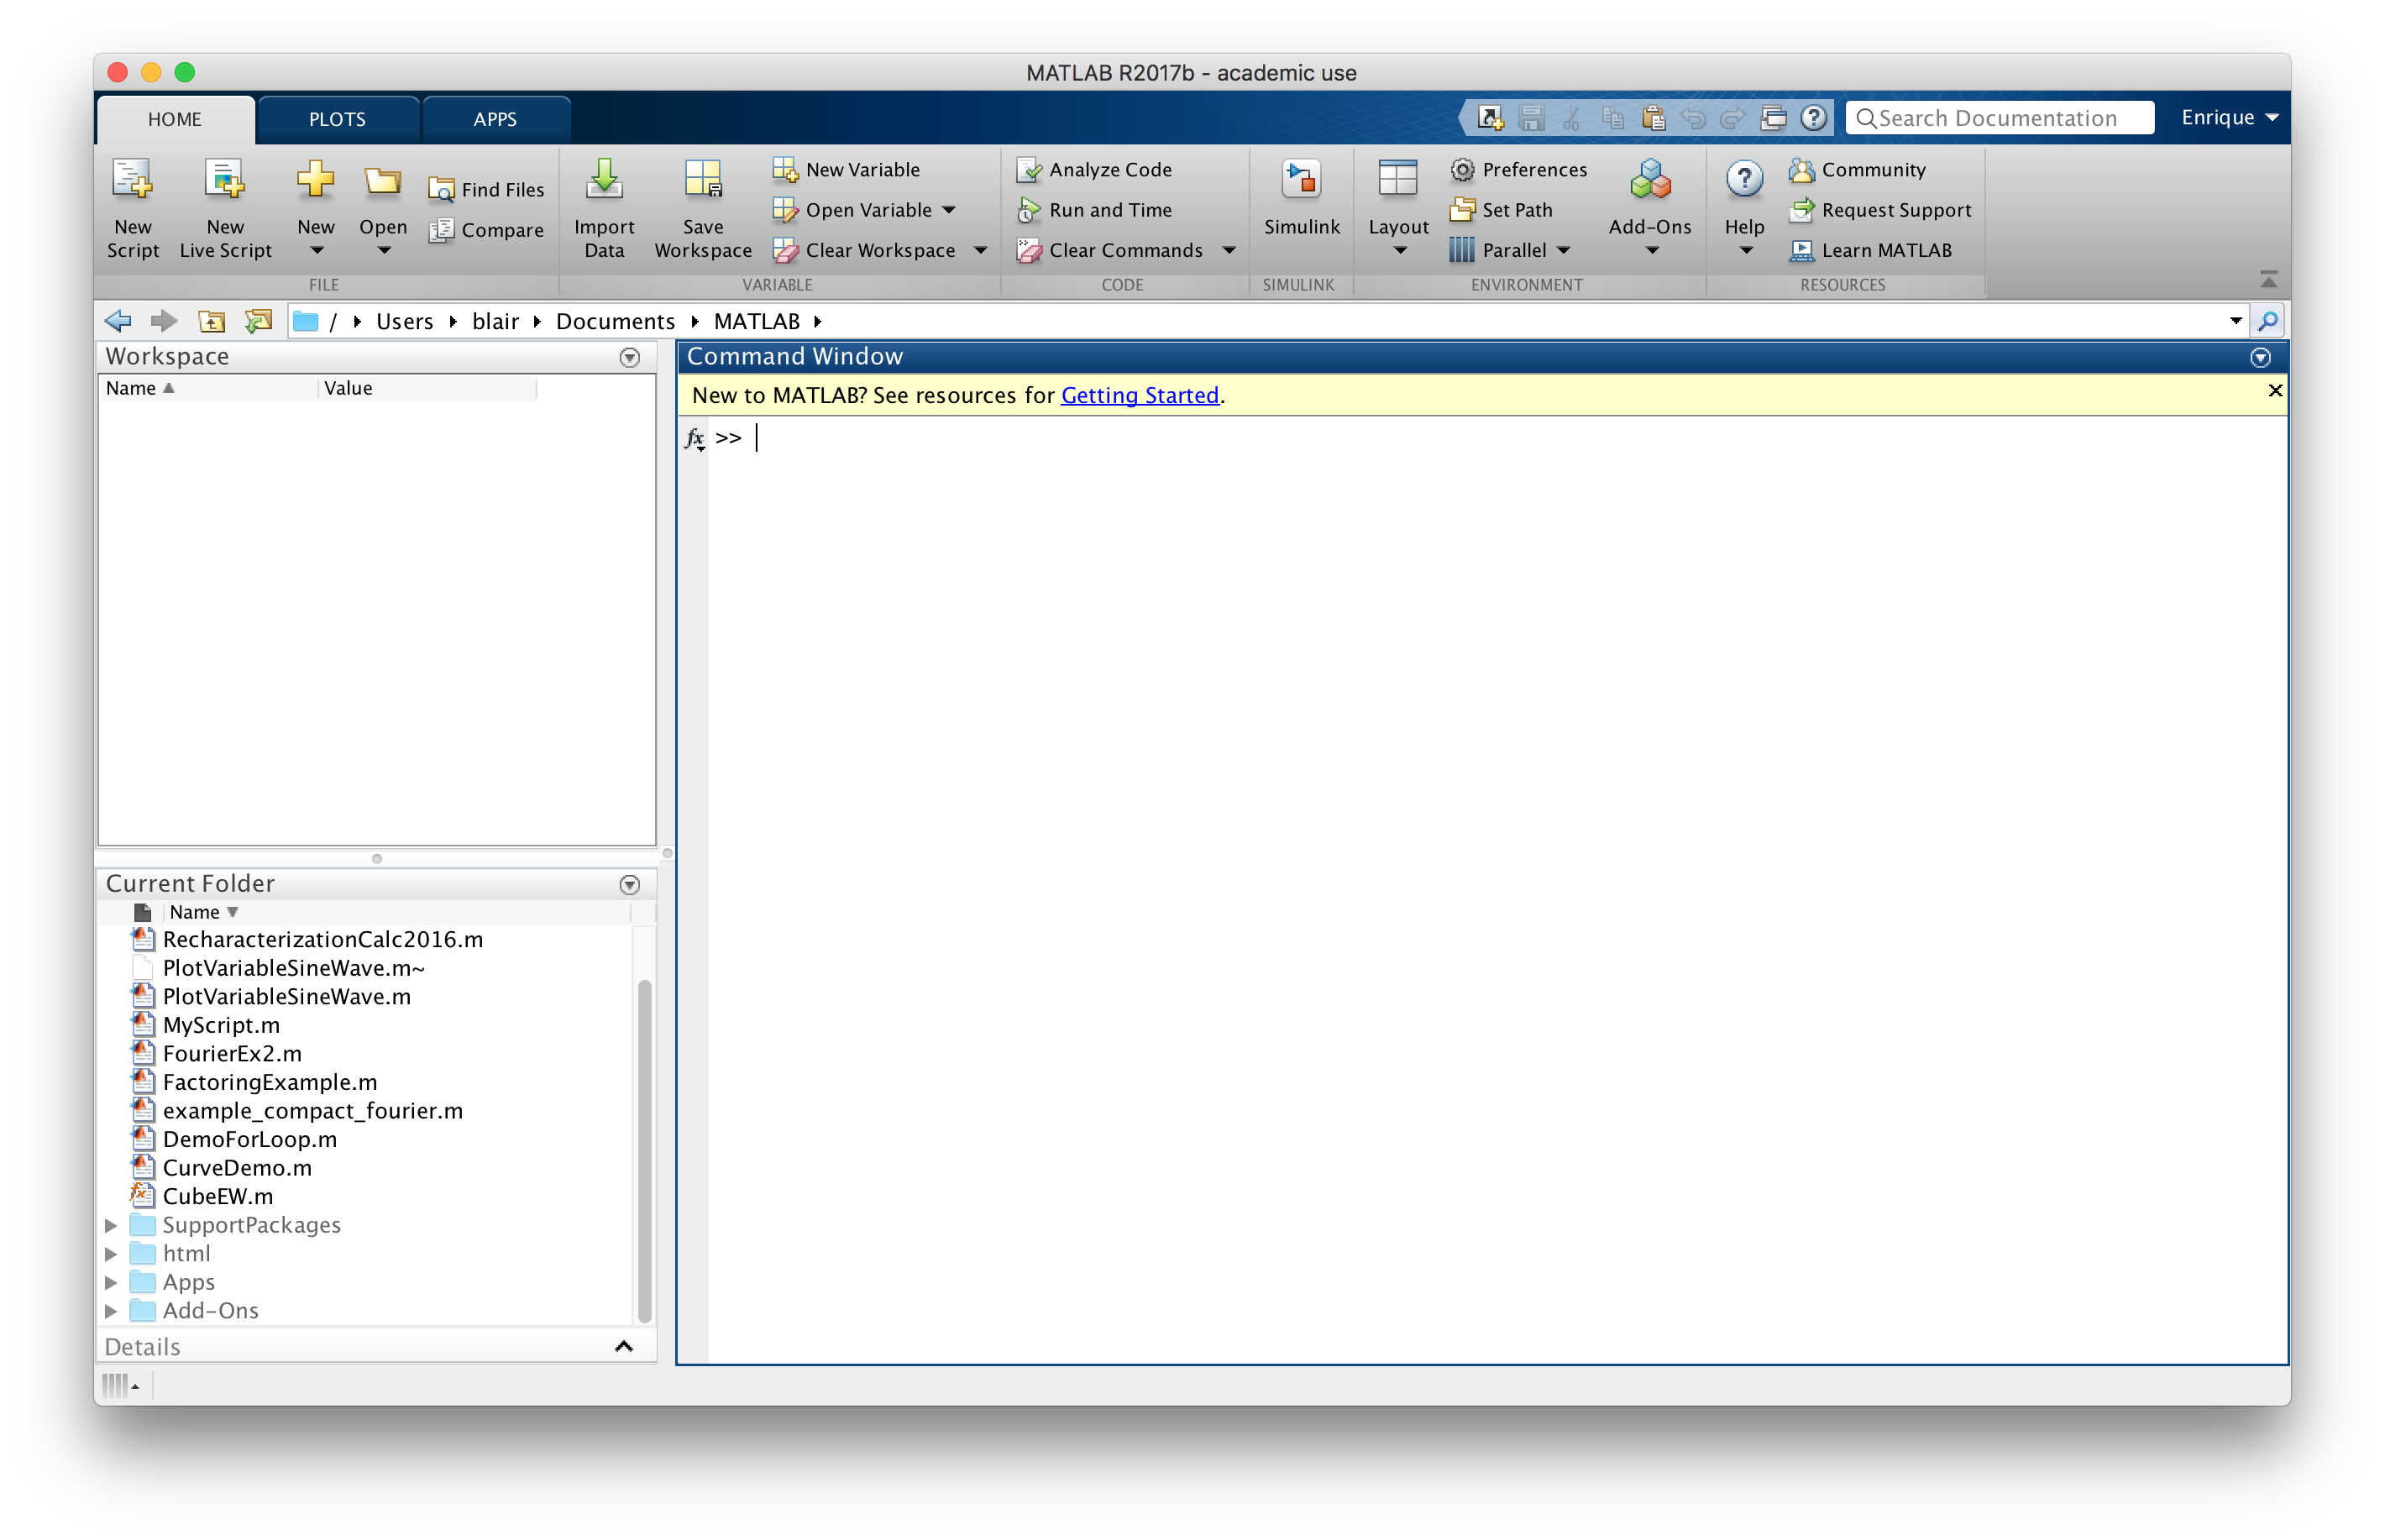
\includegraphics[width=1\textwidth]{graphics/MATLAB_Main_Window.png} 
   \caption{A typical layout for the MATLAB IDE window. It consists of three sub-windows: (1) the Command Window [right]; (2) the Workspace [upper left], and (3) the Current Folder [lower left].}
   \label{fig:MATLAB_IDE}
\end{figure}
% ^^^------------------------------------------------------------^^^

The primary and most commonly-used MATLAB user interface is the MATLAB integrated developing environment (IDE), as shown in Fig. \ref{fig:MATLAB_IDE}. This figure is customizable, but this configuration resembles the default configuration. This configuration has three windows: (1) the Command Window, (2), the Workspace, and (3) the Current Folder. We briefly describe these here:
\begin{enumerate}
\item \textbf{The Command Window}. A user types MATLAB commands at the ``\verb!>>!'' prompt. The Command Window also displays the unsuppressed text output user commands. Commands may be as simple as calculator-like arithmetic to scripts and MATLAB functions.
\item \textbf{The Workspace} lists variables, structures, and objects stored in program memory. The contents of program memory are the result of MATLAB commands and calculations.
\item \textbf{The Current Folder} lists files and subfolders contained within the current folder. The local path to the current folder is also listed in a toolbar near the top. This is important because text files define MATLAB commands, and MATLAB can only use commands associated with files found in the current folder (listed in the Current Folder window) or found within other folders stored in a special \texttt{MATLABPATH} variable. If you attempt to execute a command associated with a file not found in the current folder or in the \texttt{MATLABPATH} folders, then you will get an error in the Command Window that says ``\verb!Undefined function or variable `xxx'!,'' where ``\verb!xxx!'' is replaced by the offending command name.
\end{enumerate}

% ============================================
% ============================================
\subsection{Using MATLAB as a Calculator}
\label{subsect:MATLAB_calculator}
Perhaps the simplest way to use MATLAB is to use it as a calculator by typing mathematical operations in the Command Window. For example, at the MATLAB command prompt ``\verb!>>!'' typing ``\verb!5+6!''  followed by \texttt{RETURN} (\keys{\return}) causes MATLAB to evaluate the sum of 5 and 6. The MATLAB output is shown here:
% vvv------------------------------------------------------------vvv
\begin{lstlisting}[style=Matlab-editor, label={MATLABCalculator01}, caption={A simple addition calculation in MATLAB returns its result.}]
>> 5+6

ans =

    11

>> 
\end{lstlisting}
% ^^^------------------------------------------------------------^^^
In this code listing, line 1 begins with the prompt, ``\verb!>>!'', which is followed by the input typed by the user. MATLAB uses lines 2-6 to report that the answer, 11, is stored in the variable \verb!ans!. The re-emergence of the prompt signifies that MATLAB is ready for a new command.

Another important variation on this command is to assign the result of the mathematical operation to a variable. For example, the following results if we input ``\verb!x=5+6!'':
% vvv------------------------------------------------------------vvv
\begin{lstlisting}[style=Matlab-editor, label={MATLABCalculator02}, caption={The result of the previoius simple addition in MATLAB (see Listing \ref{MATLABCalculator02}) is stored in variable \texttt{x}.}]
>> x=5+6

x =

    11

>> 
\end{lstlisting}
% ^^^------------------------------------------------------------^^^
The command of line 1 is not a statement of equality, but rather an assignment command (we call ``\texttt{=}'' the \textit{assignment operator}). This input instructs MATLAB to evaluate the sum \verb!5+6! and store the result in the variable \texttt{x}. In lines 2-6, MATLAB reports the value that is stored in the variable \texttt{x}. Line 7 again prompts the user for a new command.

Valid MATLAB variable names may contain letters, numbers and underscores. Valid MATLAB variables may not have any spaces, nor can they begin with numbers.

Often, it is desirable to suppress the result of a MATLAB command. This can be accomplished by adding a semicolon \texttt{;} to the command, as follows:
% vvv------------------------------------------------------------vvv
\begin{lstlisting}[style=Matlab-editor, label={MATLABCalculator03}, caption={A semicolon (\texttt{;}) may be used at the end of a MATLAB command to suppress the output.}]
>> x=5+6;
>> 
\end{lstlisting}
% ^^^------------------------------------------------------------^^^
Here, the result of line 1 is suppressed, and the new MATLAB prompt indicates that MATLAB is ready to receive new command. Additionally, the \texttt{;} can be used to divide a single line into several individual commands, as follows:
% vvv------------------------------------------------------------vvv
\begin{lstlisting}[style=Matlab-editor, label={MATLABCalculator04}, caption={The result of a simple addition calculation is saved in the variable \texttt{x}, which is used for a follow-on calculation.}]
>> x=5+6;y=x*2

y =

    22

>>
\end{lstlisting}
% ^^^------------------------------------------------------------^^^
Here, the same command is issued as before, and a second command instructs MATLAB to multiply the value stored in \texttt{x} by 2, and to store the result in a second variable \texttt{y}. Since the second command did not end with a \texttt{;}, its output was not suppressed, and MATLAB reports this result as 22.

\subsubsection{MATLAB Functions}
At this point, we have used the additive and multiplicative binary operators, ``\verb!+!'' and ``\verb!*!'', respectively; as well as the assignment operator ``\verb!=!''. Other valid operators include ``\verb!-!'' (subtraction), ``\verb!/!'' (division), and ``\verb!^!'' (exponentiation). Important functions include \verb!exp()! (the exponential), \verb!sin()! (the sine function), \verb!cos()! (the cosine function) and \verb!tan()! (the tangent function). MATLAB's trigonometric functions accept arguments in radians, but the functions \verb!sind()!, \verb!cosd()!, and \verb!tand()! are degree-input versions of the other trigonometric functions.

MATLAB also recognizes certain predefined constants. We can use ``\texttt{pi}'' to represent the irrational number $\pi$, and ``\texttt{1i}'' is used to represent $i=\sqrt{-1}$. Consider the use of these constants with functions:
% vvv------------------------------------------------------------vvv
\begin{lstlisting}[style=Matlab-editor, label={MATLABCalculator05}, caption={Some examples of pre-defined constants in MATLAB.}]
>> x = cos(pi/2)

x =

   6.1232e-17

>> y = cosd(90)

y =

     0

>> z = exp(1i*pi)

z =

  -1.0000 + 0.0000i
\end{lstlisting}
% ^^^------------------------------------------------------------^^^
Here, lines 1 and 7 evaluate the cosine of $\pi/2$ and $90^\circ$. The results are stored in ``\texttt{x}''  and ``y'', respectively. Note that \texttt{cos(pi/2)} evaluates to a very small number (approximately zero), whereas \texttt{cosd(90)} evaluates to zero.

% ============================================
% ============================================
\subsection{Using MATLAB to Run Scripts}

\subsubsection{Creating a New Script}

It often is helpful to combine many commands in a single file and execute them in sequence as a script. There are several ways to make a new script. One can do any of the following:
\begin{enumerate}
\item Click the ``New Script'' button in the upper right region of the toolbar.
\item Click the ``New Document'' button in the upper right region of the toolbar, and then select ``Script''
\item Press \keys{\cmd+N} on Mac (or \keys{\ctrl+N} on a Windows keyboard)
\item Type \texttt{edit} followed by \keys{\return} in the command window. %Type ``\verb!edit scriptname.m!'' followed by \keys{\return}, where \verb!scriptname.m! is the desired script name with a ``\texttt{.m}'' extension. Note that MATLAB requires valid file names to start with a letter (not a numeral or other special character). Numbers may be included, along with the underscore ``\texttt{\_}'' but special characters and spaces are forbidden. If the script already exists, it will be opened for editing. If it does not exists, you will be asked if you wish to make a new script with the specified name.
\end{enumerate}
Each of these actions opens a new, untitled script for editing in a new Editor window, as seen in Fig.\ \ref{fig:MATLAB_IDE_with_Editor}.

% vvv------------------------------------------------------------vvv
\begin{figure}[htbp] %  figure placement: here, top, bottom, or page
   \centering
   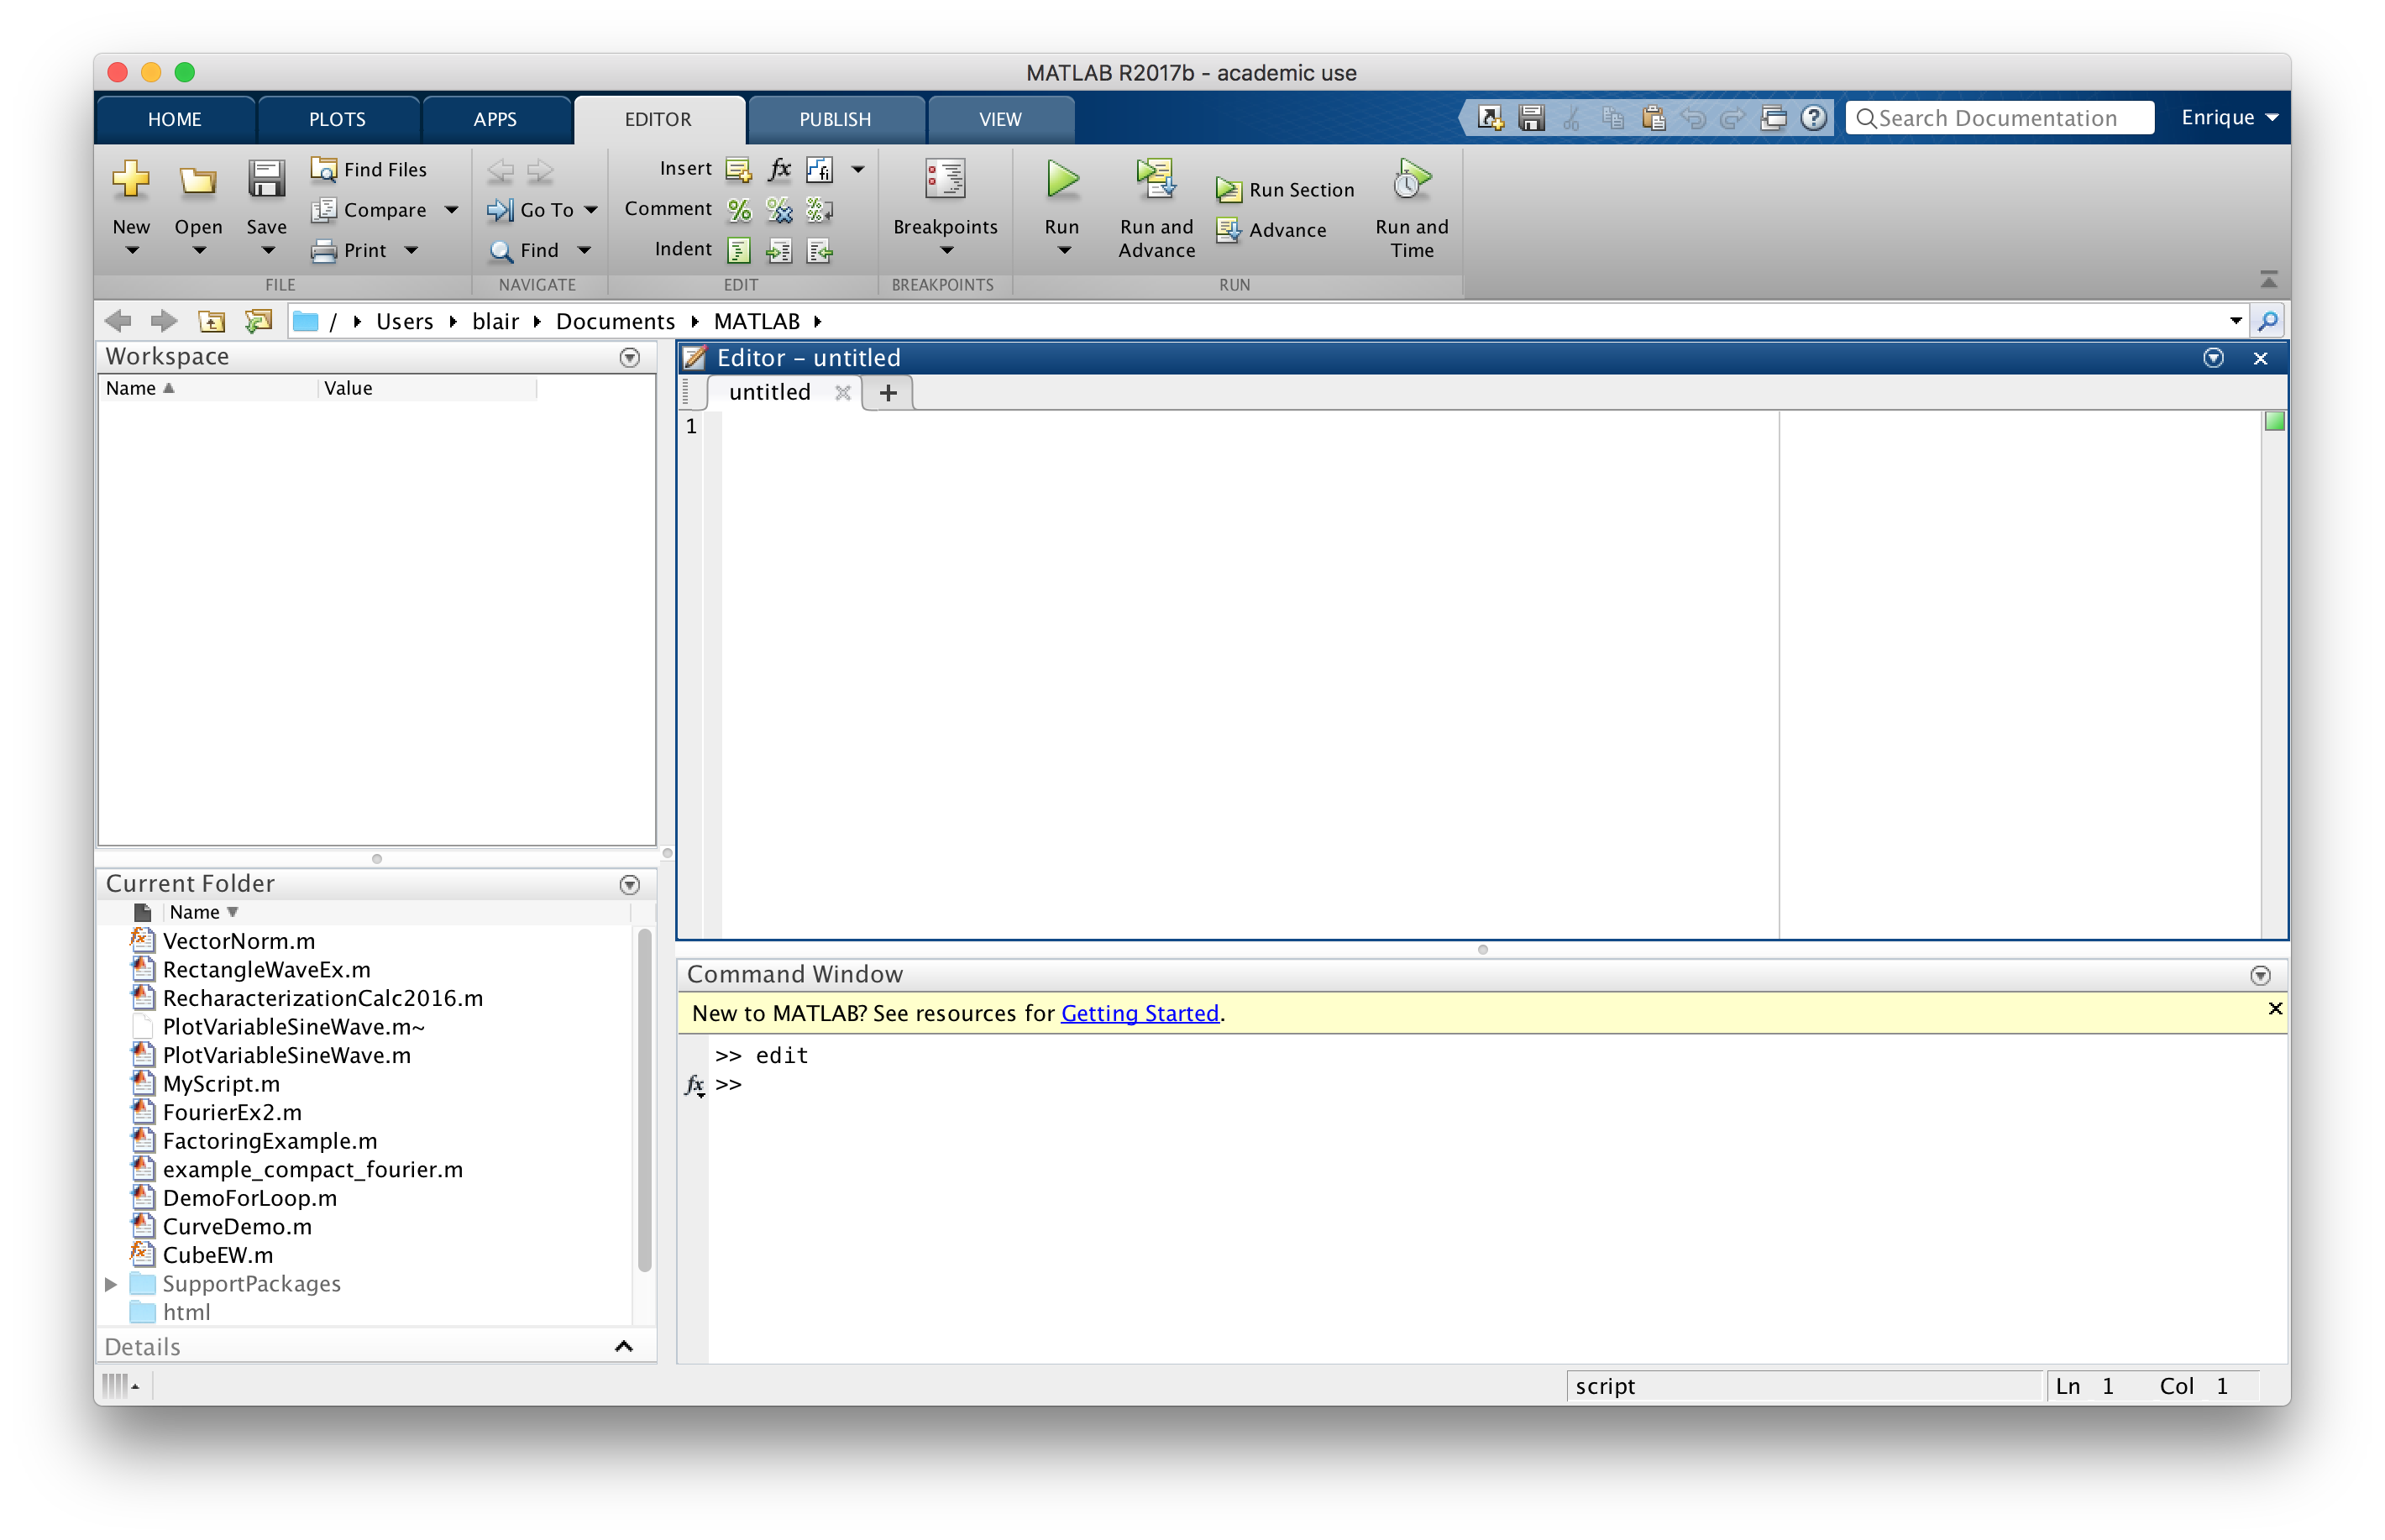
\includegraphics[width=1\textwidth]{graphics/MATLAB_Main_Window_with_Editor.png} 
   \caption{A typical layout for the MATLAB IDE window with an Editor window.}
   \label{fig:MATLAB_IDE_with_Editor}
\end{figure}
% ^^^------------------------------------------------------------^^^



\subsubsection{Writing a Script}
To write the script, write commands in the script just as in section \ref{subsect:MATLAB_calculator}. As before, use ``\texttt{;}'' to suppress output or divide a line into multiple commands. Comments may be added to any line of script by using the ``\texttt{\%}'' symbol. For a given line in the script, any text following a ``\texttt{\%}'' will be ignored and will not be evaluated as a command.

\subsubsection{Executing a Script}
To execute a script, first make sure that the file containing the script is saved in either the current folder or in a folder listed in the \texttt{MATLABPATH} variable. Then, simply type the name of the script exactly (but, without the \texttt{.m} extension) in the command line. Alternately, with the Editor as the active window and the desired script as the active tab within the Editor, click the ``\texttt{Save and Run}'' icon (green right-ward-pointing triangle) in the Editor tab of the toolbar.
